\section{Experiments}
\label{sec:exp}
We evaluate the efficiency and usefulness of {\sc GeoHighlight} in an extensive set of experiments. We consider two types of experiments: first, a performance study to measure the influence of {\em similarity}, size constraint $k$, and $tlimit$ on execution time, and second, a user study to evaluate how efficient analysts can gain insights in our framework.

\vspace{5pt}
\noindent {\bf Experiment Settings.} Unless otherwise states, we set $k = 5$, $\sigma = 0.4$, and $tlimit = 200ms$. We use New York dataset for our experiments. All experiments are implemented in Python (functionality) and JavaScript (visualization) on a 2.4GHz Intel Core i5 machine with an 8GB main memory, running OS X 10.9.2.

\begin{figure}
  \centering
  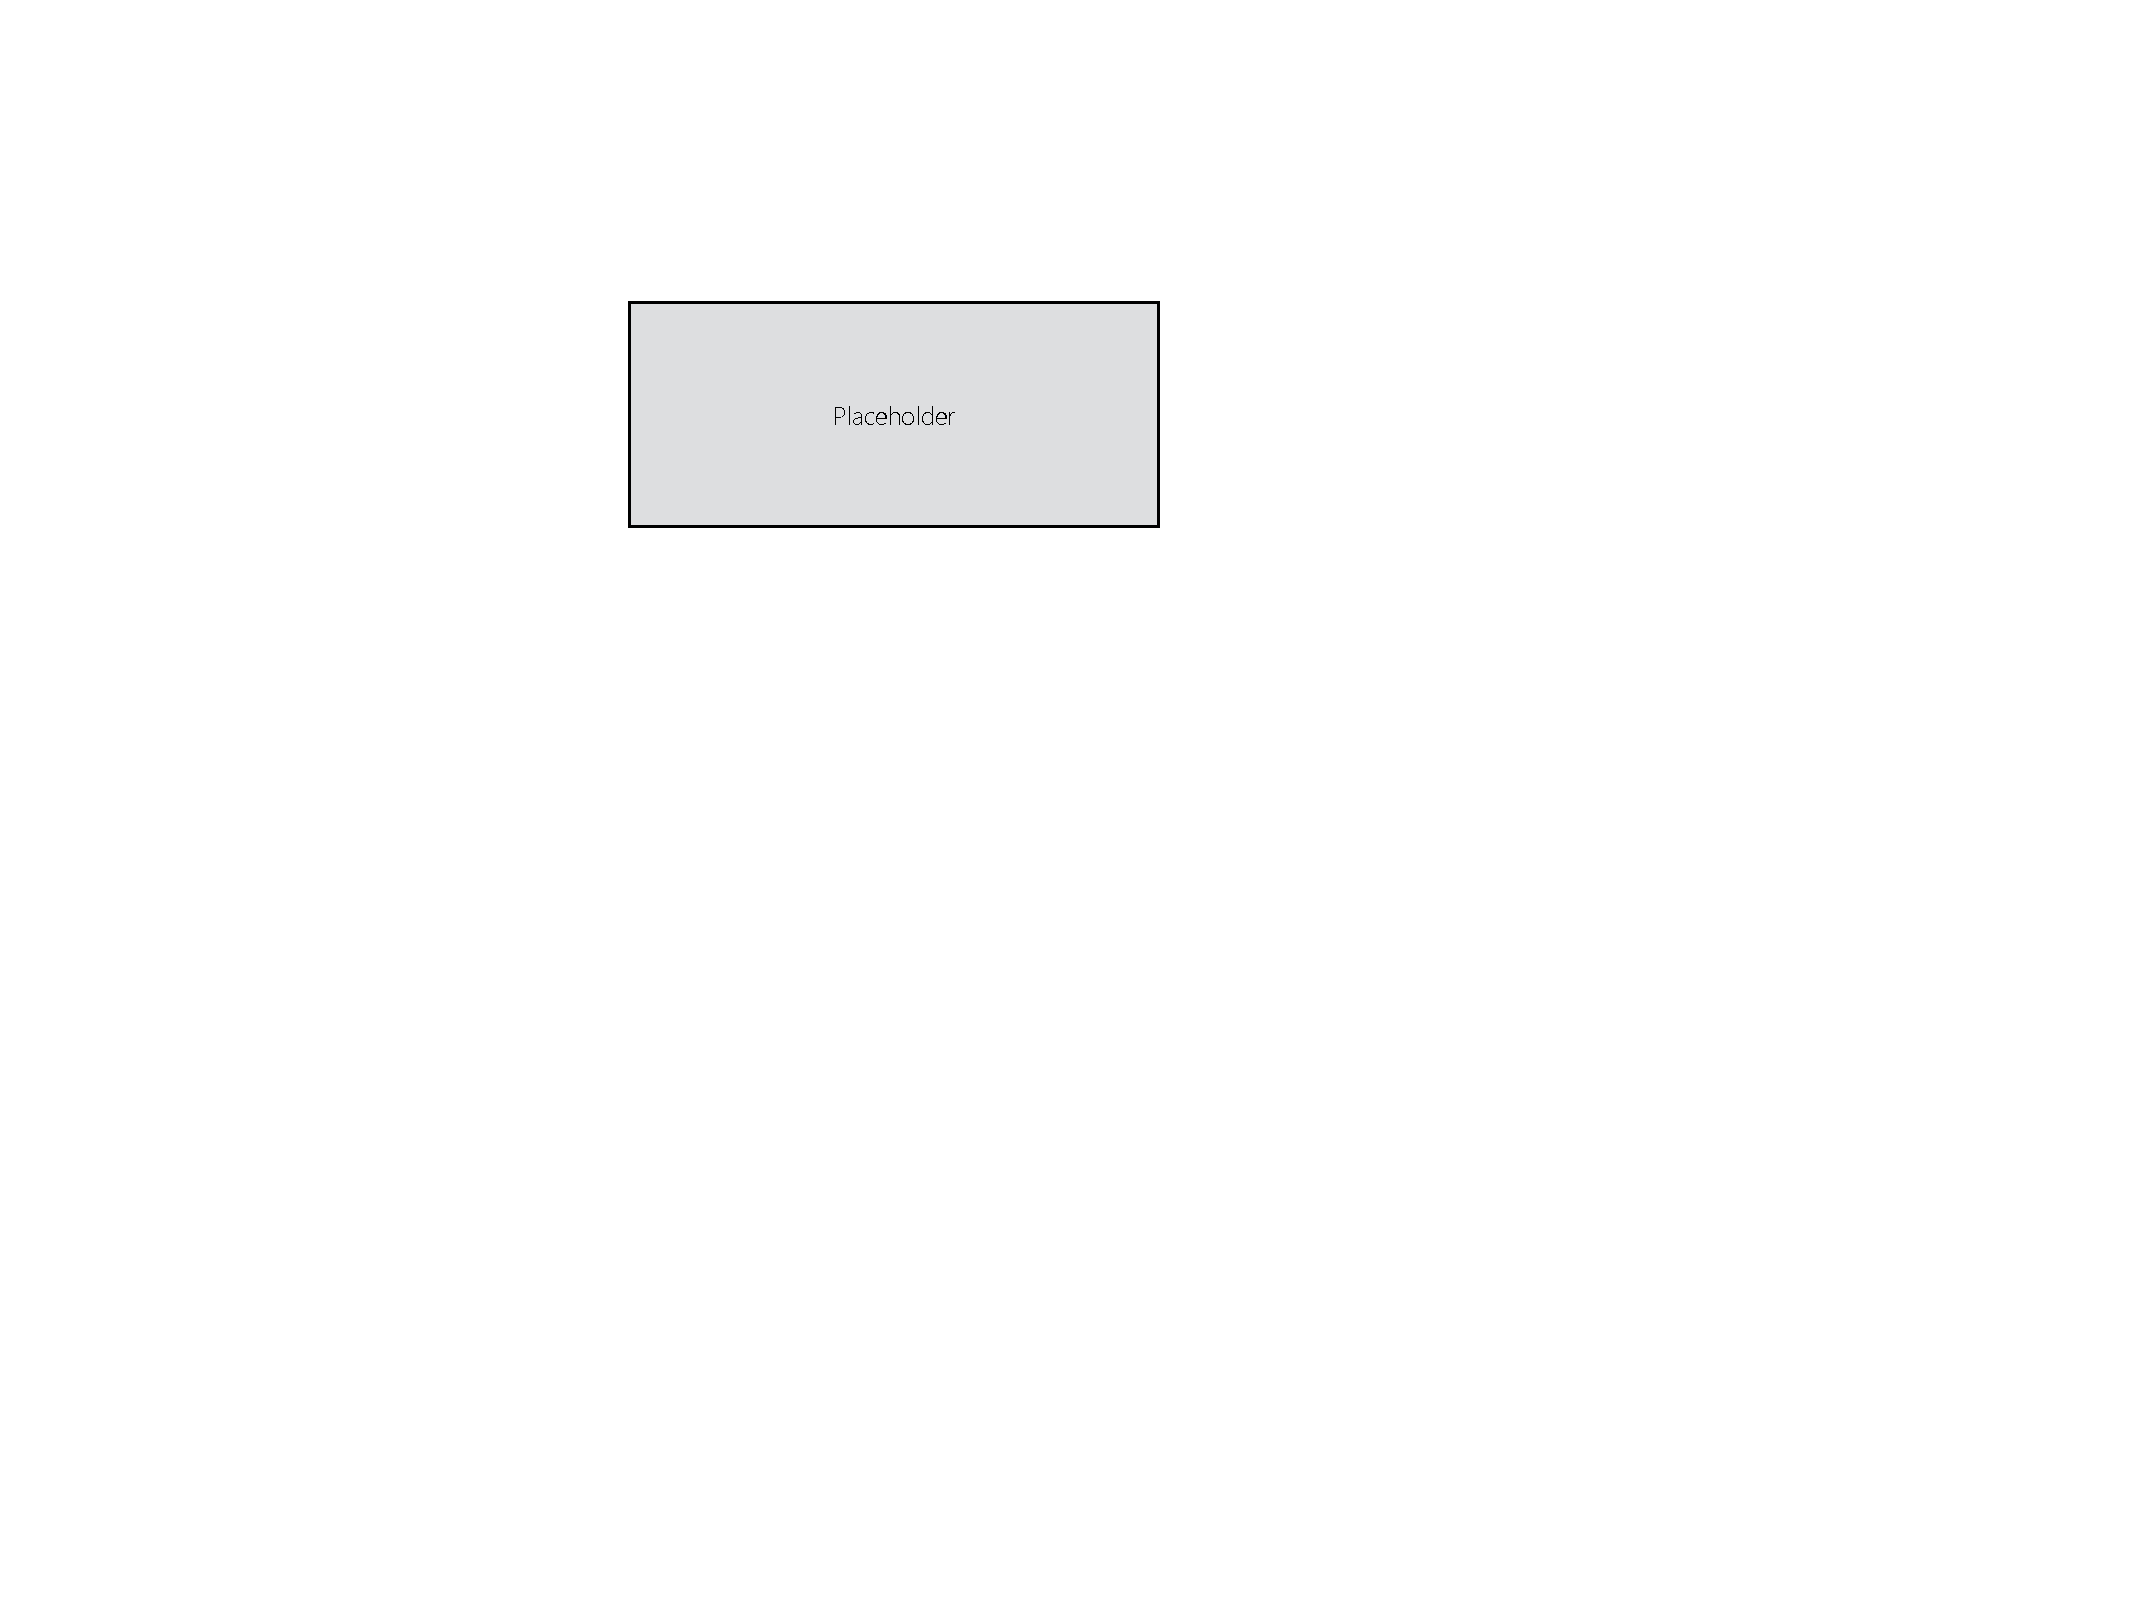
\includegraphics[width=\columnwidth]{figs/placeholder}
\caption{Performance Evaluation}
\label{fig:performance}
\end{figure}

\vspace{5pt}
\noindent {\bf Performance Study.} {\sc GeoHighlight} is designed for exploratory context where interactivity is a need. The best-effort greedy approach of {\sc Highlighter} (Algorithm \ref{algo:geoh}) guarantees to return the best possible results within a time limit. We consider a large time limit in order evaluate the effect of similarity and size constraint $k$ on execution time. Figure \ref{fig:performance} illustrates the results.

Figure \ref{fig:performance} left illustrates the effect of size constraint by varying $k$ from $2$ to $500$.

\vspace{5pt}
\noindent {\bf User Study.}